\documentclass[varwidth=true, border=2pt]{standalone}

\usepackage{pgfplots}
\usepackage{tikz}

\usetikzlibrary{calc,patterns,angles,quotes}

\begin{document}
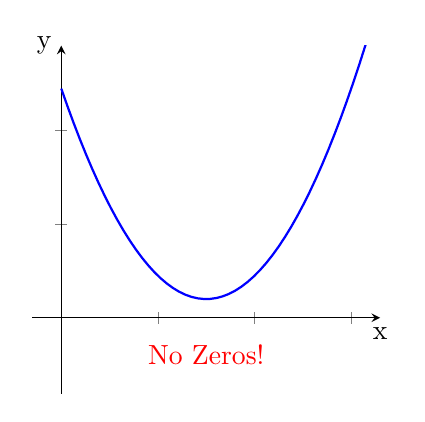
\begin{tikzpicture}
    \begin{axis}[
        legend pos=south east,
        axis x line=middle,
        axis y line=middle,
	every axis x label/.style={at={(current axis.right of origin)},anchor=north},
	every axis y label/.style={at={(current axis.above origin)},anchor=east},
	xticklabels=\empty,
	yticklabels=\empty
        grid = none ,
        width=6cm,
        height=6cm,
        grid style={dashed, gray!1},
        xmin=0,     % start the diagram at this x-coordinate
        xmax= 1.5,    % end   the diagram at this x-coordinate
        ymin=-0.25,     % start the diagram at this y-coordinate
        ymax= 1.3,   % end   the diagram at this y-coordinate
        %axis background/.style={fill=white},
        xlabel=x,
        ylabel=y,
        %xticklabels={-2,-1.6,...,2},
        %yticklabels={-8,-7,...,8},
        %tick align=outside
        enlargelimits=true,
        tension=0.08]

        \addplot[domain=-0:8, blue, thick,samples=250] {2*(x-0.75)^2 + 0.1}; % Parabola
  %      \addplot[domain=0.7:1.65, red, thick,samples=250] {1.5*x-1.25}; % Tangent Line


%	\addplot[dashed,red,mark=none] coordinates{(1.25,0)(1.25,0.625)} node[below, pos=0] {$x_0$}; %x0
%	\addplot[red, only marks, mark=*] coordinates {(0.8333,0)(1.25,0.625)};
		\node(x1)[red] at (axis cs: 0.75,-0.2){{No Zeros!}};


    \end{axis}
\end{tikzpicture}
\end{document}